\chapter{JDBC}
\label{chap:jdbc}

\fcolorbox{black}[HTML]{E9F0E9}{\parbox{\textwidth}{%
\noindent \textbf{Learning goals}\\
The junior-colleague
\begin{enumerate}[nolistsep]
\item can describe what JDBC is.
\item can explain the benefits of JPA over JDBC.
\item can identify the base interfaces of JDBC.
\item can use JDBC to connect to a database.
\item can use JDBC to query a database.
\item can use JDBC to create a table.
\item can use JDBC to insert, update, and delete records in a table.
\item can use transactions in a JDBC application.
\item can describe what SQL injection is.
\item can use Prepared Statements to prevent SQL injection.
\item can explain the ACID-properties of a transaction.
\item can explain different isolation levels and the problems that can possibly occur.
\item can explain what connection pooling is.
\item can describe what HikariCP is.
\end{enumerate}}}

\section{What is JDBC?}

The way every Java application connects to a database is through the JDBC API.
JDBC or Java (Jakarta) Database Connectivity is Java's low-level API for making database connections and handling SQL queries and responses. It's a low-level API so you have to write quite some boilerplate code.
JDBC is an adapter layer from Java to SQL. It gives Java developers a common interface for connecting to a database, issuing queries and commands, and managing responses.


\section{The database}

Use docker to supply the database in the development environment.  In case anything goes wrong, you simply recreate your environment from scratch. 
There are some advantages of using docker on your development machine: there’s less clutter on your machine and you can easily work on multiple projects with different databases and database versions. 


\section{JDBC Interfaces}

\begin{figure}[t]
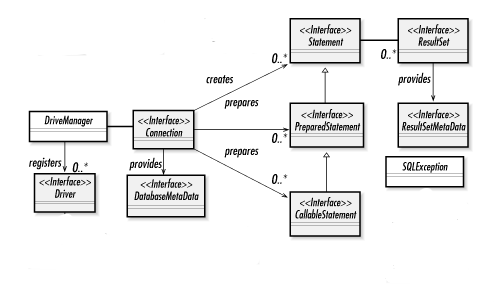
\includegraphics[width=\textwidth]{./images/jdbc/jdbc_diagram.png}
\centering
\end{figure}

\begin{figure}[t]
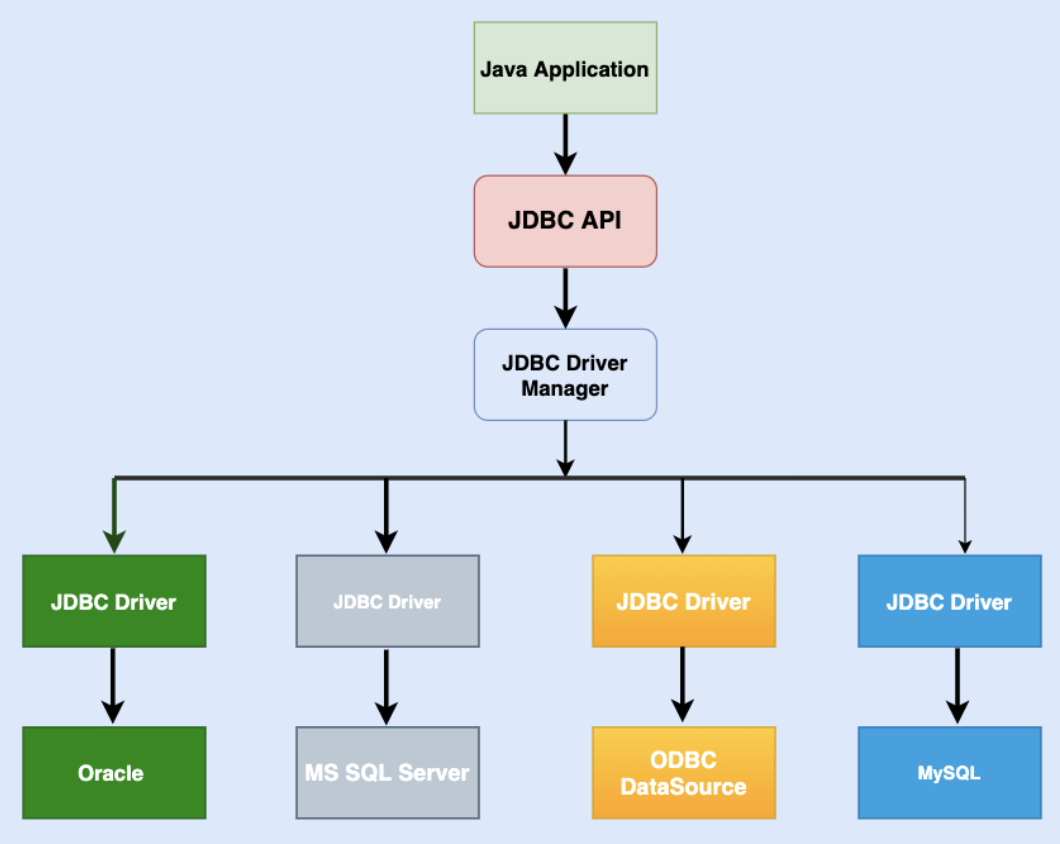
\includegraphics[width=\textwidth]{./images/jdbc/jdbc_1}
\centering
\end{figure}

\begin{lstlisting}[language=java,frame=single]
import java.sql.Connection;
import java.sql.DriverManager;
import java.sql.SQLException;
import java.sql.ResultSet;
import java.sql.Statement;
\end{lstlisting}

Each of these imports provides access to a class that facilitates the standard Java database connection:
Connection represents the connection to the database.
DriverManager obtains the connection to the database. (Another option is DataSource, used for connection pooling. )
ResultSet and Statement model the data result sets and SQL statements.
SQLException handles SQL errors between the Java application and the database.


\section{Database manipulation}
\subsection{Obtaining a database connection}

\begin{lstlisting}
try (Connection conn = 
          DriverManager.getConnection("jdbc:mysql://localhost:3306/moviedb", "user", "password")) {
        LOGGER.info("Connnection established: " + conn.getCatalog());
        LOGGER.info("Connnection established: " + conn.getMetaData().getDriverName());
     } catch (SQLException e) {
        LOGGER.fatal("Something went wrong.", e);
     }

\end{lstlisting}

The try-with-resources block ensures automatic closing of the database connection, even if exceptions occur.

The call DriverManager.getConnection() attempts to establish a connection to the specified database.  It leverages the provided connection URL and credentials to achieve this.
The connection URL "jdbc:mysql://localhost:3306/moviedb" defines the connection details.
\begin{itemize}
\item jdbc:mysql - Identifies the database type, MySQL in this case.
\item localhost - Specifies the hostname or IP address of the MySQL server
\item 3306 - Denotes the default port number for MySQL connections
\item moviedb - Represents the target database name within the MySQL server.
\item Credentials: "user" and "password" represent the username and password for a valid MySQL account with access to the moviedb database. 
\end{itemize}

If the connection is established successfully, the code proceeds to log informative messages:

\begin{itemize}
\item conn.getCatalog(): Retrieves and logs the name of the connected database catalog. In most cases, this corresponds to the database name specified in the connection URL 
\item conn.getMetaData().getDriverName(): Obtains and logs information about the JDBC driver used to establish the connection. This can be helpful for debugging purposes.
\end{itemize}


The catch (SQLException e) block acts as a safety net. If any exceptions related to SQLException arise during the connection process, this block intercepts them.

\subsection{Create a Table}

\begin{lstlisting}
package be.pxl.jdbc;

import org.apache.logging.log4j.LogManager;
import org.apache.logging.log4j.Logger;

import java.sql.Connection;
import java.sql.DriverManager;
import java.sql.SQLException;
import java.sql.Statement;

public class CreateTable {
	private static final Logger LOGGER = LogManager.getLogger(CreateTable.class);

    public static void main(String[] args) {
        try (Connection conn = DriverManager.getConnection("jdbc:mysql://localhost:3307/moviedb", "user", "password");
            Statement statement = conn.createStatement()) {
            statement.execute("CREATE TABLE employee (id INTEGER NOT NULL AUTO_INCREMENT, " +
		            "name TEXT, " +
		            "salary FLOAT, " +
		            "PRIMARY KEY (id))");
            LOGGER.info("Table 'employee' created.");
        } catch (SQLException e) {
            LOGGER.fatal("Something went wrong.", e);
        }
    }
}
\end{lstlisting}

The code showcases table creation using JDBC's Statement object and the CREATE TABLE SQL command.

\subsection{SQL Injection}


SQL injection is a code injection technique that exploits a security vulnerability occurring in the database layer of an application. It allows an attacker to insert arbitrary SQL code into a query that can be executed by the database, potentially compromising the security of the database and leaking information.

Given the movies database, let's consider a scenario where an application retrieves information about a movie based on user-provided input (e.g., movie name). The application might construct a SQL query by concatenating strings,  including the user input. If the application fails to properly sanitize the user input, it can be exploited using SQL injection.

\begin{lstlisting}
package be.pxl.jdbc;

import org.apache.logging.log4j.LogManager;
import org.apache.logging.log4j.Logger;

import java.sql.Connection;
import java.sql.DriverManager;
import java.sql.ResultSet;
import java.sql.ResultSetMetaData;
import java.sql.SQLException;
import java.sql.Statement;

public class SqlInjection {

	private static final Logger LOGGER = LogManager.getLogger(SqlInjection.class);

	public static void main(String[] args) {
		try (Connection conn = DriverManager.getConnection("jdbc:mysql://localhost:3307/moviedb", "user", "password")) {
			Statement statement = conn.createStatement();
			String movieName = "A CLOCKWORK ORANGE";
			String movieName2 = "A CLOCKWORK ORANGE' UNION SELECT *, '1', '1' FROM DIRECTOR where '1=1";
			String query = "SELECT * FROM MOVIES where MOV_TITLE = '" + movieName + "'";
			System.out.println(query);
			ResultSet resultSet = statement.executeQuery(query);
			final ResultSetMetaData meta = resultSet.getMetaData();
			final int columnCount = meta.getColumnCount();
			System.out.println("Column count: " + columnCount);
			while (resultSet.next()) {
				for (int column = 1; column <= columnCount; column++) {
					Object value = resultSet.getObject(column);
					System.out.print(value + " / ");
				}
				System.out.println();
			}
		} catch (SQLException e) {
			LOGGER.fatal("Something went wrong.", e);
		}
	}
}

\end{lstlisting}

If the application runs with user-provided movie name 'A clockwork orange' the following data is retrieved.

\begin{verbatim}
SELECT * FROM MOVIES where MOV_TITLE = 'A CLOCKWORK ORANGE'
Column count: 5
16 / A Clockwork Orange / 1971 / English / 2 / 
\end{verbatim}

\subsubsection{SQL Injection Attack to Retrieve Director Information}

An attacker could use the following input to not only retrieve movie information but also to steal the names and phone numbers of the directors: "A CLOCKWORK ORANGE' UNION SELECT *, '1', '1' FROM DIRECTOR where '1=1"

\begin{verbatim}
SELECT * FROM MOVIES where MOV_TITLE = 'A CLOCKWORK ORANGE' UNION SELECT *, '1', '1' FROM DIRECTOR where '1=1'
Column count: 5
16 / A Clockwork Orange / 1971 / English / 2 / 
1 / Alfred Hitchcock / 555-0101 / 1 / 1 / 
2 / Stanley Kubrick / 555-0102 / 1 / 1 / 
3 / Christopher Nolan / 555-0103 / 1 / 1 / 
4 / Paul Verhoeven / 555-0104 / 1 / 1 / 
5 / George Sluizer / 555-0105 / 1 / 1 / 
\end{verbatim}

The malicious input ends the original query and adds a new query. 

To prevent SQL injection, you should:
\begin{itemize}
\item Use prepared statements with parameterized queries. This ensures that user input is treated as data, not executable code.
\item Employ ORM (Object Relational Mapping) libraries, which generally use parameterized queries.
\item Validate and sanitize user input to ensure it conforms to expected formats.
\item Apply least privilege access principles to your database operations. For instance, the application's database user should not have more privileges than it needs to perform its tasks.
\end{itemize}

\section{CRUD}

Here's an  example demonstrating CRUD (Create, Read, Update, Delete) operations for tjhe "employee" table in a MySQL database using JDBC:

\begin{lstlisting}
package be.pxl.jdbc;

import org.apache.logging.log4j.LogManager;
import org.apache.logging.log4j.Logger;

import java.sql.Connection;
import java.sql.DriverManager;
import java.sql.PreparedStatement;
import java.sql.ResultSet;
import java.sql.SQLException;
import java.util.Optional;

public class EmployeeCRUD {

	private static final Logger LOGGER = LogManager.getLogger(EmployeeCRUD.class);

	private static final String url = "jdbc:mysql://localhost:3307/moviedb";
	private static final String username = "user";
	private static final String password = "password";

	public static void createEmployee(Connection connection, String name, float salary) throws SQLException {
		String query = "INSERT INTO employee (name, salary) VALUES (?, ?)";
		PreparedStatement preparedStatement = connection.prepareStatement(query);
		preparedStatement.setString(1, name);
		preparedStatement.setFloat(2, salary);
		preparedStatement.executeUpdate();
		LOGGER.info("Employee '" + name + "' created.");
	}

	public static Optional<Employee> getEmployee(Connection connection, int id) throws SQLException {
		String query = "SELECT * FROM employee WHERE id = ?";
		PreparedStatement preparedStatement = connection.prepareStatement(query);
		preparedStatement.setInt(1, id);
		ResultSet resultSet = preparedStatement.executeQuery();

		if (resultSet.next()) {
			int retrievedId = resultSet.getInt("id");
			String retrievedName = resultSet.getString("name");
			double retrievedSalary = resultSet.getDouble("salary");
			Employee employee = new Employee(retrievedId, retrievedName);
			employee.setSalary(retrievedSalary);
			return Optional.of(employee);
		} else {
			LOGGER.info("Employee with ID " + id + " not found.");
			return Optional.empty();
		}
	}

	public static void updateEmployee(Connection connection, int id, String name, float salary) throws SQLException {
		String query = "UPDATE employee SET name = ?, salary = ? WHERE id = ?";
		PreparedStatement preparedStatement = connection.prepareStatement(query);
		preparedStatement.setString(1, name);
		preparedStatement.setFloat(2, salary);
		preparedStatement.setInt(3, id);
		int rowsUpdated = preparedStatement.executeUpdate();
		if (rowsUpdated > 0) {
			LOGGER.info("Employee with ID " + id + " updated.");
		} else {
			LOGGER.info("Employee with ID " + id + " not found (update failed).");
		}
	}

	public static void deleteEmployee(Connection connection, int id) throws SQLException {
		String query = "DELETE FROM employee WHERE id = ?";
		PreparedStatement preparedStatement = connection.prepareStatement(query);
		preparedStatement.setInt(1, id);
		int rowsDeleted = preparedStatement.executeUpdate();
		if (rowsDeleted > 0) {
			LOGGER.info("Employee with ID " + id + " deleted.");
		} else {
			LOGGER.info("Employee with ID " + id + " not found (delete failed).");
		}
	}

	public static int countEmployees(Connection connection) throws SQLException {
		String query = "SELECT COUNT(*) FROM employee";
		PreparedStatement preparedStatement = connection.prepareStatement(query);
		ResultSet result = preparedStatement.executeQuery();
		if (result.next()) {
			return result.getInt(1);
		}
		return 0;
	}

	public static void main(String[] args) {
		try (Connection connection = DriverManager.getConnection(url, username, password)) {
			createEmployee(connection, "John Doe", 75000.0f);
			createEmployee(connection, "Jane Smith", 82000.5f);

			getEmployee(connection, 1).ifPresent(System.out::println);
			updateEmployee(connection, 2, "Jane Doe", 85000.0f);
			getEmployee(connection, 2).ifPresent(System.out::println);
			System.out.println("Number of employees: " + countEmployees(connection));
			deleteEmployee(connection, 1);
			System.out.println("Number of employees: " + countEmployees(connection));

		} catch (SQLException e) {
			System.err.println("An error occurred. " + e.getMessage());
			e.printStackTrace();
		}
	}
}
\end{lstlisting}

Executing the program after the employee table is created, will produce the following log messages.

\begin{verbatim}
11:57:25.825 [main] INFO  be.pxl.jdbc.EmployeeCRUD - Employee 'John Doe' created.
11:57:25.835 [main] INFO  be.pxl.jdbc.EmployeeCRUD - Employee 'Jane Smith' created.
Employee{id=1, name='John Doe', salary=75000.0}
11:57:25.868 [main] INFO  be.pxl.jdbc.EmployeeCRUD - Employee with ID 2 updated.
Employee{id=2, name='Jane Doe', salary=85000.0}
Number of employees: 2
11:57:25.885 [main] INFO  be.pxl.jdbc.EmployeeCRUD - Employee with ID 1 deleted.
Number of employees: 1
\end{verbatim}


ResultSet represents the result set of a query that retrieves data from the database.
It's a one-way cursor, meaning you can only iterate through the results once in a forward direction.
Always check if resultSet.next() returns true before trying to access column data to avoid errors.
resultSet.next() moves the cursor to the next result. It returns true if there's a next row, false if the end is reached.
Retrieving data from a result in the ResultSet starts at column 1 (not 0). You can access column data using methods like getInt(columnIndex), getString(columnIndex), etc., specifying the desired column number.



\section{Transactions}


Transactions are a mechanism to group multiple database operations into a single unit. These operations are treated as all-or-nothing:

\begin{itemize}
\item Success: If all the operations in the transaction succeed, the changes are permanently applied to the database through a commit.
\item Failure: If any operation fails due to errors (e.g. data integrity violation), the entire transaction is rolled back using rollback, undoing all the changes attempted within that transaction.
\end{itemize}

Imagine a scenario where you want to give an employee a raise. This could involve updating two tables in your database:
\begin{itemize}
\item Employee Table: Update the employee's salary field.
\item Salary History Table: Insert a new record reflecting the raise amount and date.
\end{itemize}

To ensure both updates happen successfully or neither happens at all, we can use a transaction.

\begin{lstlisting}
package be.pxl.jdbc;

import org.apache.logging.log4j.LogManager;
import org.apache.logging.log4j.Logger;

import java.sql.Connection;
import java.sql.DriverManager;
import java.sql.SQLException;
import java.sql.Statement;
import java.time.LocalDate;
import java.time.format.DateTimeFormatter;

public class SalaryRaise {

	private static final DateTimeFormatter FORMAT = DateTimeFormatter.ofPattern("yyyy-MM-dd");
	private static final Logger LOGGER = LogManager.getLogger(EmployeeCRUD.class);
	private static final String URL = "jdbc:mysql://localhost:3307/moviedb";
	private static final String USERNAME = "user";
	private static final String PASSWORD = "password";

	public static void main(String[] args) {
		try (Connection connection = DriverManager.getConnection(URL, USERNAME, PASSWORD)) {
			// Turn off auto-commit to manage transactions manually
			connection.setAutoCommit(false);
			try {
				Statement statement = connection.createStatement();
				statement.executeUpdate("UPDATE employee SET salary = salary * 1.1 WHERE id = 2");
				statement.executeUpdate("INSERT INTO salary_history (employee_id, salary_raise, date) VALUES (2, 10, '" + FORMAT.format(LocalDate.now()) + "')");
				// If both updates succeed, commit the transaction
				connection.commit();
				System.out.println("Salary raise successful!");
			} catch (SQLException e) {
				// If any error occurs, rollback the transaction (undo changes)
				connection.rollback();
				System.out.println("Salary raise failed: " + e.getMessage());
			}
		} catch (SQLException e) {
			LOGGER.error("A database error occurred. " + e.getMessage());
		}

	}
}
\end{lstlisting}

We disable auto-commit using setAutoCommit(false).
We perform the updates for both tables within a try block.
If both updates succeed, commit finalizes the changes.
If any SQLException occurs (e.g., insufficient privileges, data type mismatch), the catch block executes rollback to undo all changes within the transaction.
This ensures that either both tables are updated reflecting the raise, or none are updated at all, maintaining data integrity.


\textbf{ACID} stands for Atomicity, Consistency, Isolation, and Durability. These are essential properties that guarantee data integrity and consistency in database transactions (like the salary raise example you saw). 

\begin{itemize}
\item \textbf{Atomicity}: This ensures the transaction is treated as a single unit of work. Either all the operations within the transaction succeed, or none of them do. 

\item \textbf{Consistency}: This guarantees the transaction moves the database from one valid state to another. It enforces the database's defined rules and constraints. 

\item \textbf{Isolation}: This ensures concurrent transactions from multiple users don't interfere with each other. 

\item \textbf{Durability}: This guarantees that once a transaction commits, the changes are permanent and persist even in case of system failures (like power outages). The database system ensures the updates are written to stable storage (like a disk) to survive such incidents.
\end{itemize}

\section{Transaction Isolation Level}


Isolation levels in transactions play a crucial role in managing concurrency, which refers to how multiple transactions access and modify data simultaneously in a database. While concurrency improves performance by allowing multiple users to work with the database, it can also lead to data inconsistencies if not handled properly.

\textbf{Isolation Levels} define the visibility of uncommitted changes made by one transaction to other concurrent transactions. Different isolation levels offer varying degrees of data consistency at the expense of performance. Here are some common isolation levels and related phenomena:

\begin{itemize}
\item \textbf{Read Uncommitted}: This allows a transaction to read data even if it's not yet committed by another transaction. This can lead to \textbf{dirty reads}, where a transaction reads data that is later rolled back, resulting in seeing inconsistent data.

\item \textbf{Read Committed}: This allows a transaction to read data only after it's committed by another transaction. This prevents dirty reads, but can introduce \textbf{non-repeatable reads}. Here, a transaction might read the same data twice and get different results if another transaction modifies the data in between those reads.

\item \textbf{Repeatable Read}: This ensures a transaction can read the same data multiple times and get the same results, even if another transaction commits changes in between those reads. However, it can lead to \textbf{phantom reads}, where a transaction might not see data inserted by another transaction after it started its own read operation.

\item \textbf{Serializable}: This is the most stringent level, ensuring transactions are serialized (executed one after another) as if there were no concurrency. It eliminates all the anomalies mentioned above (dirty reads, non-repeatable reads, phantom reads) but has the worst performance impact.
\end{itemize}

\begin{figure}[H]
  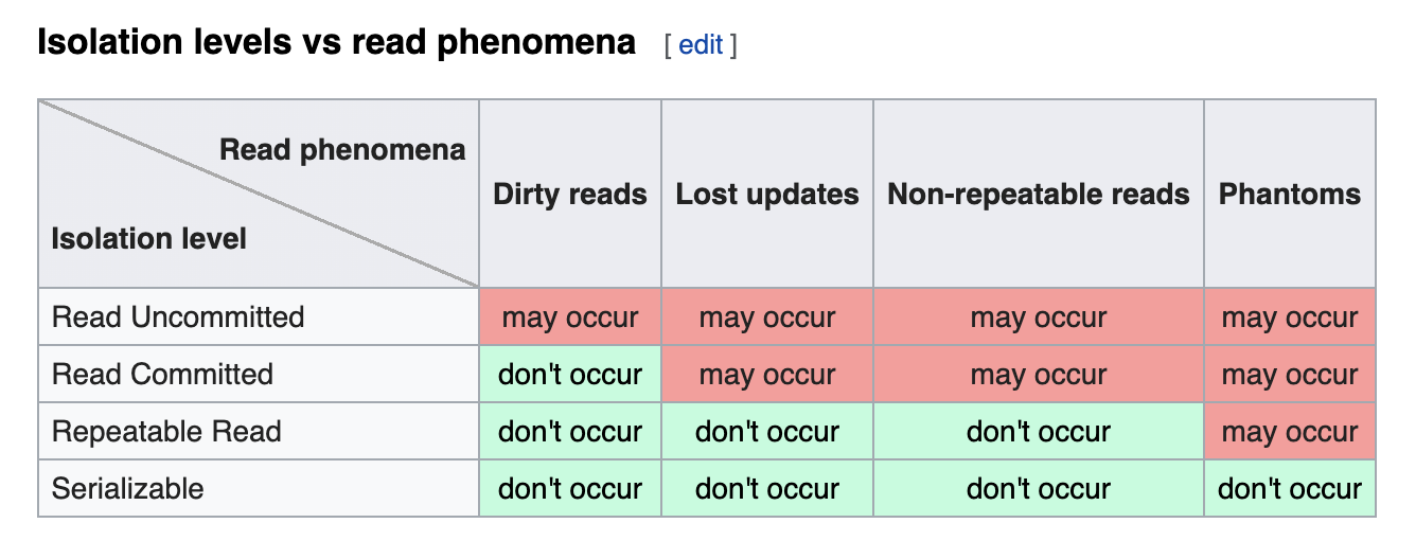
\includegraphics[width=\linewidth]{images/jdbc/isolation_levels.png}
  \caption{Isolation Levels}
  \label{fig:paths}
\end{figure}


\subsubsection{Dirty Read}

\begin{figure}[H]
  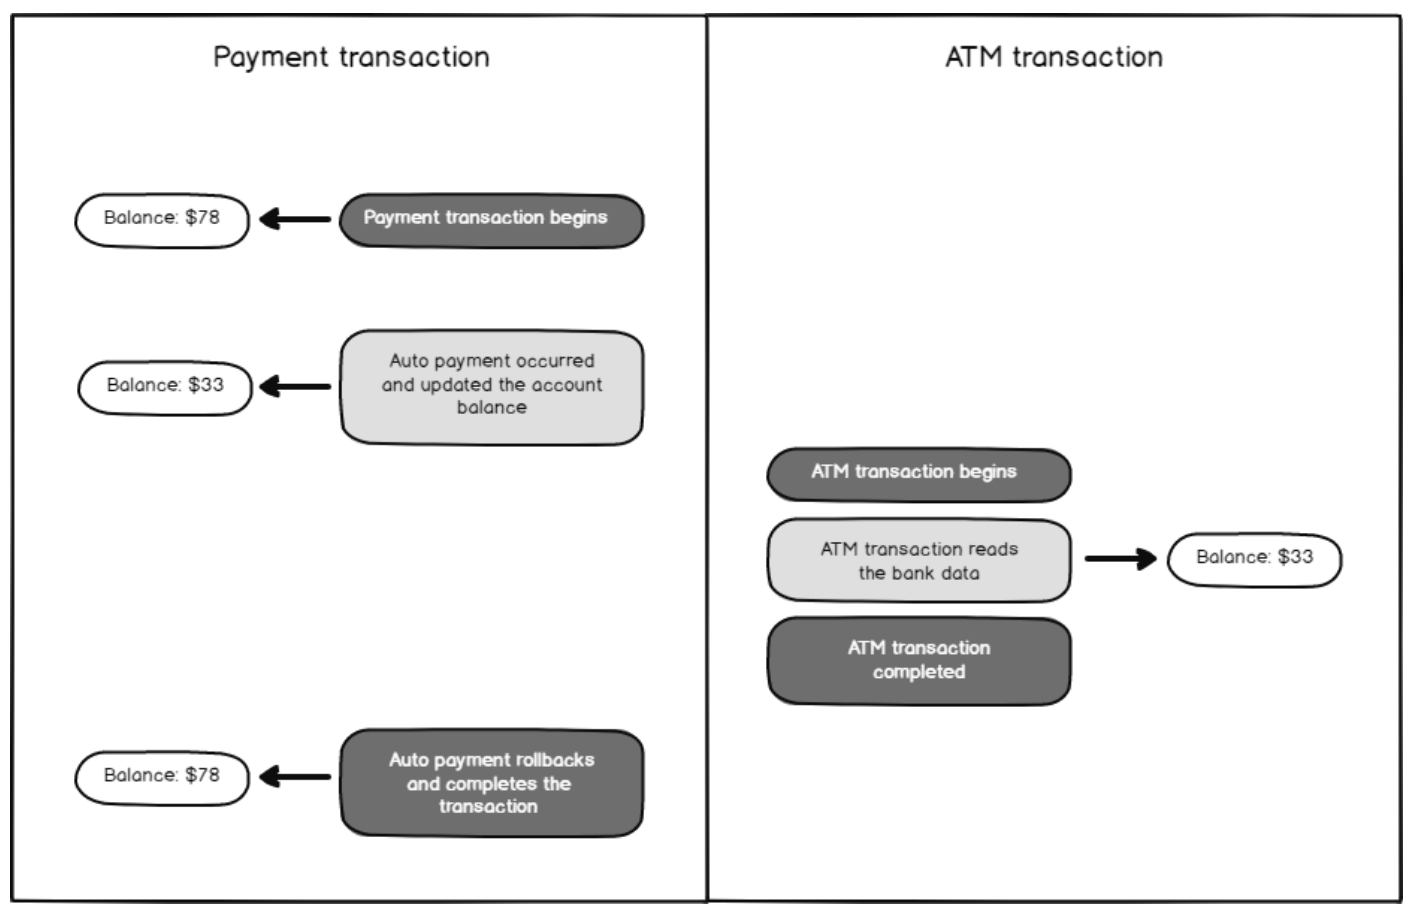
\includegraphics[width=\linewidth]{images/jdbc/dirty_read.png}
  \caption{Dirty Read}
  \label{fig:paths}
\end{figure}

A dirty read occurs when a transaction reads data that has been modified by another transaction, but that modification hasn't been committed yet. Imagine reading a friend's draft message before they send it - you see unfinalized information.

\subsubsection{Non-Repeatable Read}

Non-repeatable reads happen when a transaction reads the same data twice within its execution, and the data has changed in between due to another committed transaction. 

\begin{figure}[H]
  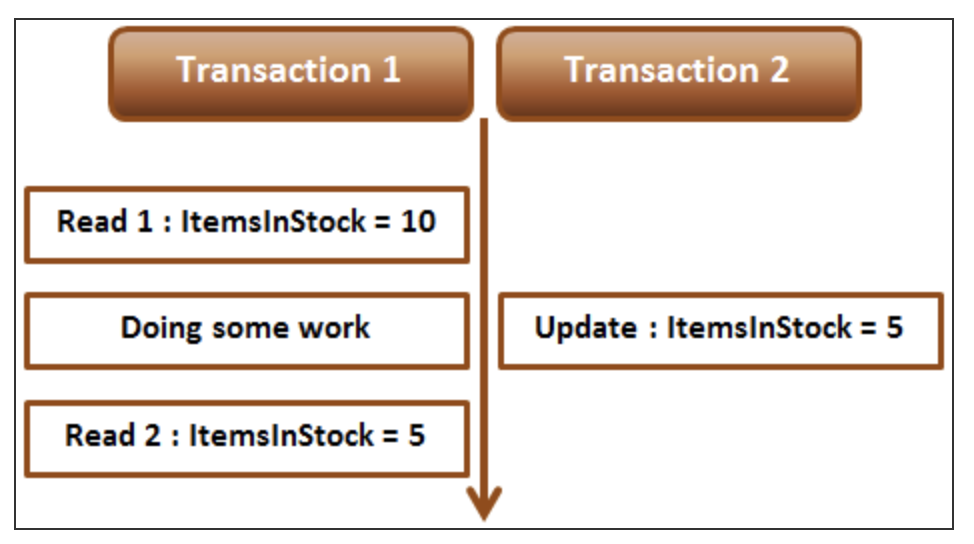
\includegraphics[width=\linewidth]{images/jdbc/non_repeatable_read.png}
  \caption{Non-Repeatable Read - Transaction 1 starts first,  reads ItemsInStock and gets a value of 10. Transaction 1 is doing some work and at this point transaction 2 starts and updates ItemsInStock to 5. Transaction 1 then makes a new read. At this point transaction 1 gets a value of 5,  resulting in non-repeatable read problem. }
  \label{fig:paths}
\end{figure}


\subsubsection{Lost update}

Lost update isn't directly an isolation level issue, but a concurrency problem. It occurs when two transactions try to modify the same data piece simultaneously, and due to isolation levels, only one update succeeds, effectively "losing" the other update.


\begin{figure}[H]
  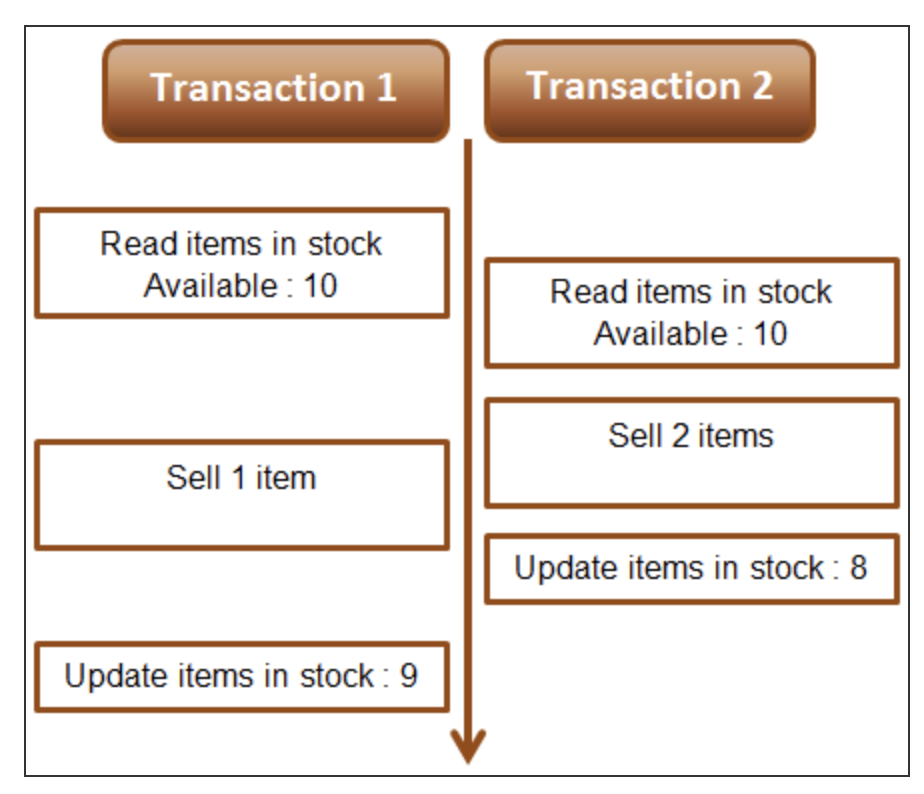
\includegraphics[width=\linewidth]{images/jdbc/lost_update.png}
  \caption{Lost Update - Transaction 1 silently overwrites the update of Transaction 2. This is called the lost update problem.}
  \label{fig:paths}
\end{figure}

\subsubsection{Phantom Read}

Phantom Read occurs when a transaction reads data that wasn't there when it started its read operation, but another committed transaction inserted that data in between. 

\begin{figure}[H]
  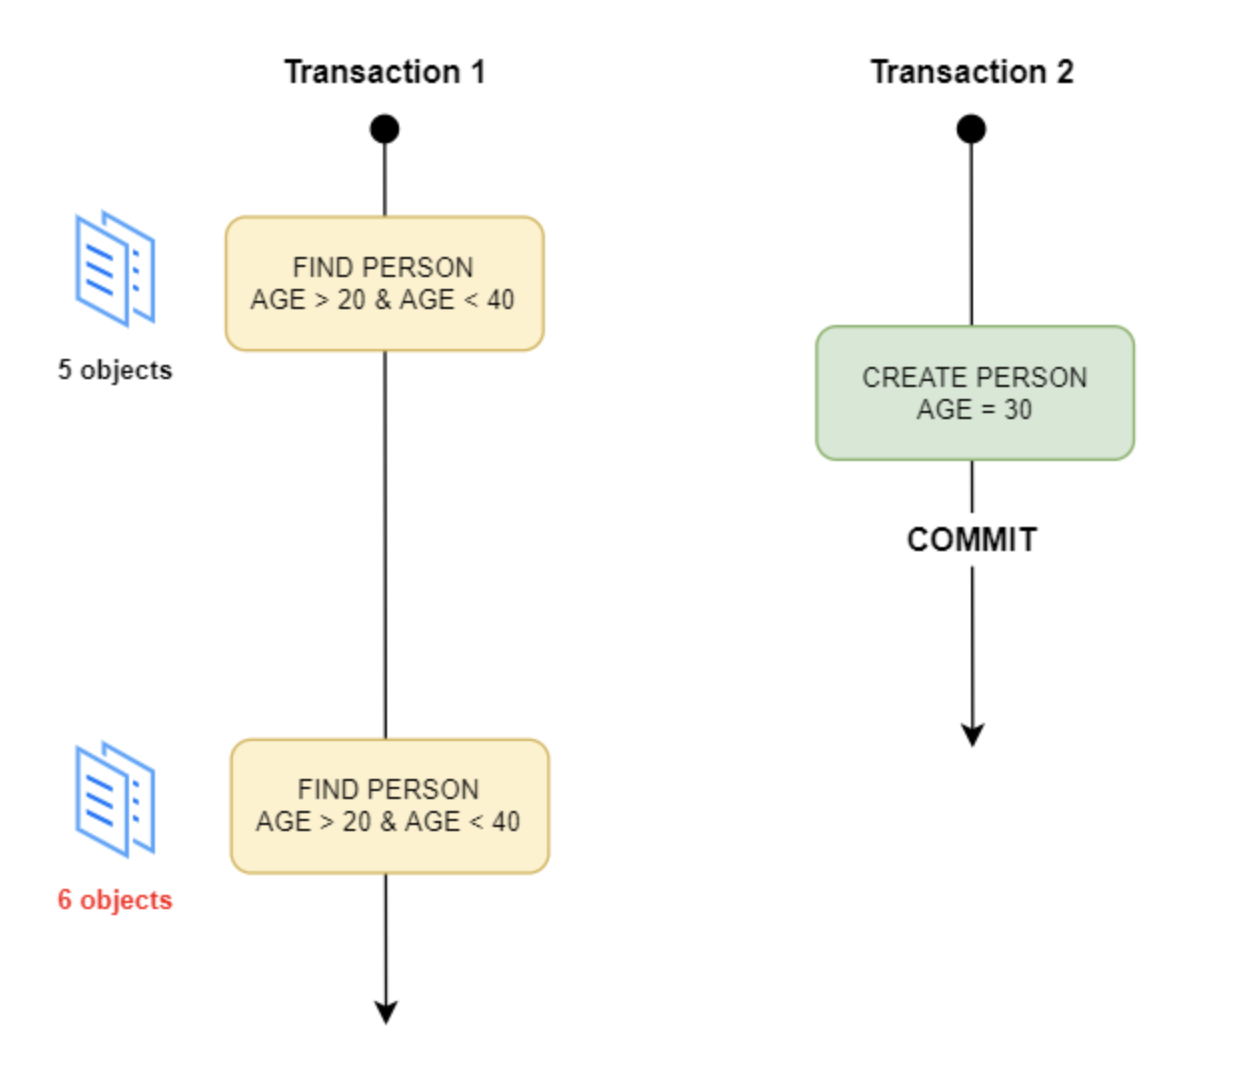
\includegraphics[width=\linewidth]{images/jdbc/phantom_read.png}
  \caption{Phantom Read}
  \label{fig:paths}
\end{figure}


Non-Repeatable Read deals with existing data being modified by another transaction after the first read while Phantom Read deals with entirely new data being inserted by another transaction that the first read hasn't seen.

Choosing the right isolation level depends on the specific needs of your application. Here's a general guideline:

\begin{itemize}
\item High Consistency: If data consistency is paramount and occasional performance slowdowns are acceptable, choose Read Committed or Repeatable Read.

\item High Concurrency: If performance is crucial and some data inconsistencies are tolerable, consider Read Uncommitted (use with caution!).
\end{itemize}

Serializable offers the strongest consistency but at the cost of significant performance overhead. Use it when absolutely necessary.


\subsection{Example}

This program will update data in the database and may or may not commit the changes immediately, depending on the scenario you want to illustrate.

\begin{lstlisting}
package be.pxl.jdbc;

import java.sql.Connection;
import java.sql.DriverManager;
import java.sql.SQLException;
import java.sql.Statement;

public class UpdaterProgram {

	static final String DB_URL = "jdbc:mysql://localhost:3307/moviedb";
	static final String USER = "user";
	static final String PASS = "password";

	public static void main(String[] args) {

		try (Connection conn = DriverManager.getConnection(DB_URL, USER, PASS)) {
			conn.setAutoCommit(false);

			try (Statement stmt = conn.createStatement()) {
				String sqlUpdate = "UPDATE employee SET salary = salary + 1000 WHERE id = " + args[0];
				stmt.executeUpdate(sqlUpdate);
				System.out.println("Data updated but not committed yet. Sleeping for 10 seconds...");
				// Sleep to allow time for the ReaderProgram to run and attempt to read the uncommitted data.
				Thread.sleep(10000);

				if ("commit".equals(args[1])) {
					conn.commit();
					System.out.println("Commit");
				} else {
					conn.rollback();
					System.out.println("Rollback");
				}
			}
		} catch (SQLException | InterruptedException e) {
			e.printStackTrace();
		}
	}
}

\end{lstlisting}


This program will attempt to read data from the database.  Depending on the isolation level set and whether the Updater Program has committed its changes, the Reader Program may see different results.

\begin{lstlisting}
package be.pxl.jdbc;

import java.sql.Connection;
import java.sql.DriverManager;
import java.sql.ResultSet;
import java.sql.SQLException;
import java.sql.Statement;

public class ReaderProgram {

	static final String URL = "jdbc:mysql://localhost:3307/moviedb";
	static final String USER = "user";
	static final String PASS = "password";

	public static void main(String[] args) {
		try (Connection conn = DriverManager.getConnection(URL, USER, PASS)) {
			// Set the isolation level here, for example:
			conn.setTransactionIsolation(Connection.TRANSACTION_READ_UNCOMMITTED);

			try (Statement stmt = conn.createStatement()) {
				String sql = "SELECT * FROM employee WHERE id = " + args[0];
				ResultSet rs = stmt.executeQuery(sql);

				while (rs.next()) {
					int id = rs.getInt("id");
					String name = rs.getString("name");
					double salary = rs.getDouble("salary");

					System.out.println("ID: " + id + ", Name: " + name + ", Salary: " + salary);
				}
			}
		} catch (SQLException e) {
			e.printStackTrace();
		}
	}
}
\end{lstlisting}

Start the UpdaterProgram. This program will update a row but will not commit immediately. It sleeps for 10 seconds, allowing you to start the ReaderProgram within this window.

Run the ReaderProgram.  Depending on the isolation level you set in the Reader Program, it may or may not see the uncommitted changes made by the UpdaterProgram. You should run the Reader Program multiple times, each time setting a different isolation level to observe how each level affects the visibility of uncommitted changes.

\begin{itemize}
\item TRANSACTION\_READ\_UNCOMMITTED: The Reader Program will see the uncommitted changes.
\item TRANSACTION\_READ\_COMMITTED (and higher levels): The Reader Program will not see the uncommitted changes.
\end{itemize}


\section{Connection pooling}
Opening and closing database connections like you did above with the DriverManager.getConnection method takes some time.

Especially in web applications, you do not want to open up a fresh database connection for every single user request, rather you want to have a small pool of connections that are always open and shared between users.

That’s what JDBC connection pools are for.  A connection pool keeps open a small number of database connections (think: 10) and instead of opening up database connections yourself, you’ll ask the connection pool to give you one of these (10) connections.



HikariCP is the recommended connection pool to use in your Java application. However, you have plenty possibilities to choose from.
HikariCP is also Spring Boot’s default choice. Use Oracle’s UCP, if you are working with Oracle databases.

All of these connection pools are  solid, performant, and offer sane defaults and error handling.

Independent of the option you choose, you will then, in your JDBC code, not open up connections yourself through the DriverManager, but rather you will construct a connection pool, represented by the DataSource interface, and ask it to give you one of its connections.



\begin{lstlisting}
package be.pxl.jdbc;

import com.zaxxer.hikari.HikariDataSource;
import org.apache.logging.log4j.LogManager;
import org.apache.logging.log4j.Logger;

import javax.sql.DataSource;
import java.sql.Connection;
import java.sql.PreparedStatement;
import java.sql.ResultSet;
import java.sql.SQLException;
import java.util.Optional;

public class ConnectionPoolExample {
    private static final Logger LOGGER = LogManager.getLogger(ConnectionPoolExample.class);

    private static final String URL = "jdbc:mysql://localhost:3307/moviedb";
    private static final String USERNAME = "user";
    private static final String PASSWORD = "password";

    public static Optional<Employee> getEmployee(Connection connection, int id) throws SQLException {
        String query = "SELECT * FROM employee WHERE id = ?";
        PreparedStatement preparedStatement = connection.prepareStatement(query);
        preparedStatement.setInt(1, id);
        ResultSet resultSet = preparedStatement.executeQuery();

        if (resultSet.next()) {
            int retrievedId = resultSet.getInt("id");
            String retrievedName = resultSet.getString("name");
            double retrievedSalary = resultSet.getDouble("salary");
            Employee employee = new Employee(retrievedId, retrievedName);
            employee.setSalary(retrievedSalary);
            return Optional.of(employee);
        } else {
            LOGGER.info("Employee with ID " + id + " not found.");
            return Optional.empty();
        }
    }

    public static void main(String[] args) throws SQLException {
        DataSource dataSource = createDataSource();

        try (Connection connection = dataSource.getConnection()) {
            getEmployee(connection, 2).ifPresent(System.out::println);
        }
    }

    private static DataSource createDataSource() {
        HikariDataSource ds = new HikariDataSource();
        ds.setJdbcUrl(URL);
        ds.setUsername(USERNAME);
        ds.setPassword(PASSWORD);
        return ds;
    }
}
\end{lstlisting}


